\documentclass[letterpaper,twocolumn,10pt]{article}
\usepackage{usenix}
\usepackage{endnotes}
\usepackage[tight]{subfigure}

\usepackage{url}
\usepackage{multirow}
\usepackage{array}
\usepackage{epsfig}
\usepackage{footnote}
\usepackage{amsmath}
\widowpenalty=10000
\clubpenalty=10000

\begin{document}

\title{\Large \bf On the Design and Implementation of Structured P2PVPNs}

\author{
David Isaac Wolinsky$^{\ast}$,
Linton Abraham$^{\bullet}$,
Kyungyong Lee$^{\ast}$,
Yonggang Liu$^{\ast}$,
\\
Jiangyan Xu$^{\ast}$,
P. Oscar Boykin$^{\ast}$,
Renato Figueiredo$^{\ast}$
\\
$^{\ast}$University of Florida, 
$^{\bullet}$Clemson University
\\
}

\maketitle

%\thispagestyle{empty}

\subsection*{Abstract}
%\begin{sloppypar}
In recent years, there have been a multitude of P2P VPNs primarily falling
into two categories: 1) P2P communication but centralized session management and
2) use of unstructured P2P systems.  These tend to reduce the overhead in
creating a VPN and allow users to directly connect bypassing the overhead of
communicating through a third party proxy.  This significantly improves upon
classical, centralized VPNs, though it adds a new complexity as the approaches
have varying scalability constraints.  To address this, we propose a run-time
decentralized P2P model using a structured P2P system.  In this paper, we
will describe the components of this model as well as present and evaluate our
reference implementation. Our approach provides an intuitive and simplistic
setup, reduces the requirements for connectivity, offers better proxy selection
in lieu of NAT traversal, and provides an opportunity for more intuitive trust
solutions. For evaluation, we will compare system and networking overheads of
the different VPN technology focusing on latency, bandwidth, and memory.
%\end{sloppypar}

\section{Introduction}
A Virtual Private Network (VPN) provides the illusion of a Local Area Network
(LAN), namely direct communication, over a wide area network such as the
Internet while guaranteeing secure and authenticated communication amongst
participants.  Common uses of VPNs include accessing company or academic
network resources while traveling abroad, playing LAN based video games over the
Internet, connecting distributed resources from multiple sites, and securing
your Internet traffic while in unsecure locations.  In the context of this
paper, we focus on VPNs that provide connectivity between individual resources
and so all resources that need symmetric connectivity will need to be
configured with VPN software.  Our work is significantly different than others
which define VPNs `` as the 'emulation of a private Widea Area Network (WAN)
facility using IP facilities' (including the public Internet or private IP
backbones).''~\cite{ip_vpns}.  Those VPNs tend to be clustered where a single
site may have a few virtual routers and many nodes on a subnet unique to the
rest of the VN, these virtual routers  are connected to other environments
similarly configured systems.

Centralized VPNs enable distributed connectivity but at the cost of maintaining
a central server, which becomes the conduit for all traffic, becoming a
performance bottleneck and can make end-to-end security complicated.
To alleviate this, there have been three directions 1) support for multiple VPN
servers for a single VPN~\cite{openvpn, cloudvpn}, 2) the use of P2P
connections for bypassing central communication that rely on run-time central
authentication \cite{hamachi, wippien}, and 3) the use of unstructured P2P
networks to form VPNs based upon shared secrets without user authentication and
limitations on network size~\cite{p2pvpn, n2n, tinc}.  In this paper, we present
a novel approach to forming secure, scalable, efficient, and self-configuring VPNs
through the the use of Structured P2P systems that has no reliance on
centralized systems after initialization.  Structured P2P technology enables
users to communicate directly with all users without knowing anything beyond
their virtual IP bypassing the need for centralization while providing
all-to-all communication without maintaining all-to-all connectivity with
participants.  Interesting applications of P2P include efficient wide area
multicast, data distribution, storage, chat applications, and even IP
connectivity.

Current generation P2PVPNs do not scale well, provide features such as
full-tunneling of network traffic, such as forwarding Internet traffic, nor do
they have intuitive ability for scalable multicast or broadcast.  P2PVPNs rely
on direct connectivity and in general will not work if NAT (Network Address
Translation) traversal between peers is unsuccessful.  Unstructured P2P based
VPNs have similar issues, though have the ability to reuse the unstructured
overlay to relay packets though with scalability constraints as this requires
complete knowledge of the system, all-to-all connectivity, or use of broadcast
messages to find a destination.  Furthermore, current unstructured P2P systems 
lack the ability to police participants in the system.

The problems we seek to address with our P2PVPN model include:
%\small {
\begin{itemize}
\setlength{\itemsep}{0pt}
\setlength{\parskip}{0pt}
\item reducing the role of centralization for user authentication in a VPN
\item managing participants in a live system
\item supporting full-tunneling of Internet traffic in a P2P system
\item handling relay selection in lieu of unsuccessful NAT traversal
\item supporting multicast and broadcast communication
\item debugging a P2P overlay
\end{itemize}
%}
A rudimentary overview of our solutions to the above problems follows and will
be covered in depth in the rest of this paper.  To provide fully decentralized
run-time connectivity and policing, we use an automated certificate authority based
upon the use of user groups.  In the case of full-tunneling, P2PVPNs introduce
significantly more complexity since a simple routing table swap as done in
central VPNs no longer work, as such we investigate three different mechanisms
for tunneling all Internet traffic to our full-tunnel endpoint(s) besides our
P2P traffic.  When nodes cannot directly communicate, they seek to connect to
peers that are mutually physically close to each other and use them to relay
communication.  For efficient multicast and broadcast communication, we rely on
the use of bootstrapping a private P2P system whose members are only
participants of the VPN.

Explicitly, our contributions made in this paper are:
%\small{
\begin{itemize}
\setlength{\itemsep}{0pt}
\setlength{\parskip}{0pt}
\item automated group-based certificate authority
\item three different approaches to configuring full-tunneling
\item intelligent selection of relays
\item use of a private P2P VPN system bootstrapped of a general P2P system
\item discussion of our techniques used for discovering bugs in our system
\end{itemize}
%}

We would like to note that many of our contributions are not novel by themselves,
but rather, it is the culmination of these components and their interaction,
namely a model of a structured P2P VPN, that is our novel contribution for
this paper.

The rest of this paper is organized as follows.  Section II gives an overview
of current VPN technologies and the efforts to decentralized.  Section III
introduces P2P structures and our previous work IPOP (IP over P2P).  Section IV
describes the contributions of this paper, namely a feature-full P2PVPN.  In
Section V, we discuss our implementation and present evaluation comparing
centralized, P2P, and our VPN.  Finally, we give some concluding remarks in
Section VI.

\section{Virtual Private Networks}
There exist many different flavors of virtual networking, this paper focuses on
those that are used to create or extend a virtual layer 3 network.  A few
examples of such technologies include Cisco's Systems VPN and AnyConnect VPN
Client~\cite{ciscovpn} as well as OpenVPN~\cite{openvpn}.  In this section, we
begin by going in depth on client configuration of VPNs followed by sections
describing different VPN server configurations as highlighted in
Table~\ref{tab:vpn_types}.  Finally we conclude the section by presenting a
Table~\ref{tab:vpns}, which presents actual VPN products stating the VPN server
type and presenting some qualitative overview.


\begin{table}[ht]
\label{tab:vpn_types}
\setlength{\itemsep}{0pt}
\setlength{\parskip}{0pt}
\centering
\begin{tabular}[c]{|m{2cm}|m{4.5cm}|} \hline
Type & Description \\ \hline
Centralized & Clients communicate through one or more servers which are statically
configured \\ \hline
Decentralized Servers & Clients communicate through one ore more servers which are
dynamically configured \\ \hline
Centralized Servers / P2P Clients & Servers provide authentication, session management, and
optionally relay support while peers attempt to communicate directly with each
other, i.e., P2P links \\ \hline
Unstructured P2P & No distinction between clients and servers, members either know
the entire network or use broadcast to discover routes between each other \\ \hline
Structured P2P & No distinction between clients and servers, members are usually
within $O(\log N)$ hops of each other via a greedy routing algorithm \\ \hline
\end{tabular}
\caption{VPN Classifications}
\end{table}

\subsection{Client VPN Configuration}
\label{clientvpn}
In Figure~\ref{fig:vpn}, we abstract the common features of all VPNs with focus
on the client.  The key components of the client are 1) client software that
communicates with the VPN overlay directly and 2) a virtual network device.
During initialization VPN software begins by authenticating with some overlay
agent, optionally it then queries the agent for information about the network
such as the network address space, and then starts the virtual network device.

\begin{figure}[ht]
\centering
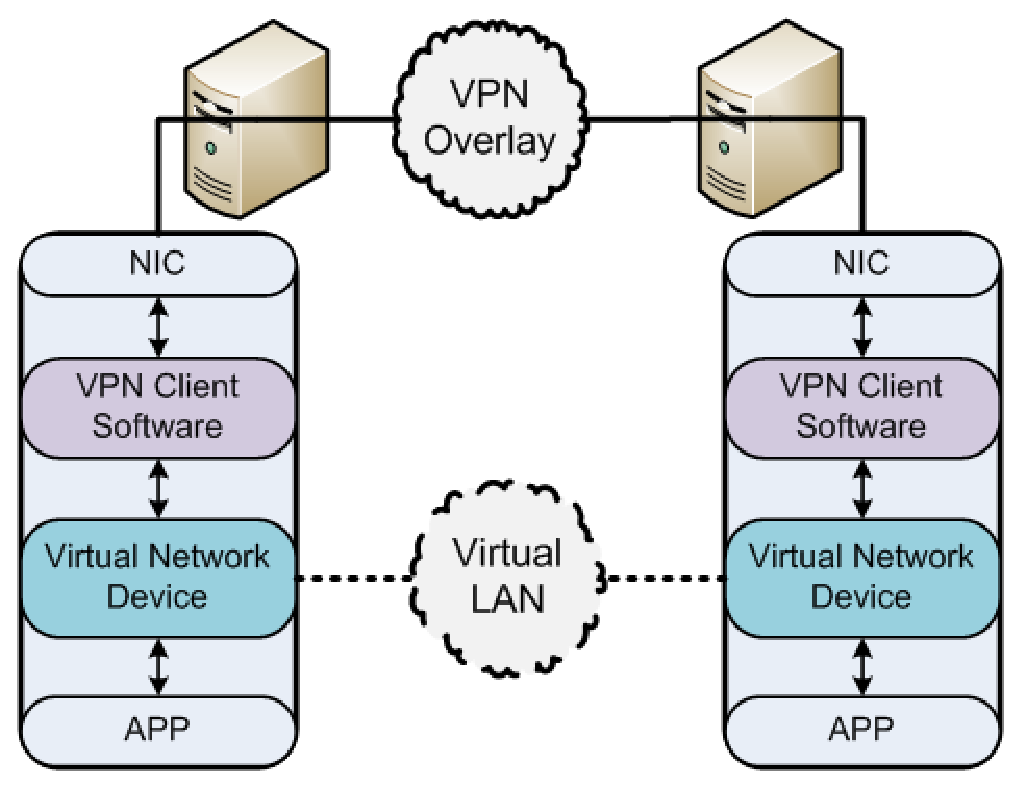
\epsfig{file=figs/vpn.png.eps, width=3in}
\caption{A typical VPN client.  The VPN uses a virtual network device to make
interaction with the virtual network transparent.  Packets that are destined
for virtual network destinations are sent via routing rules to the virtual
network device, which acts as like a file descriptor read and written to by the
VPN client.  The VPN client in turn sends and receives packets over the hosts
physical (real) network device.}
\label{fig:vpn}
\end{figure}

There are many different mechanisms for communicating with the overlay agent.
For quick setup, a system may provide a shared secret password or key that is
common for the entire network.  A more user-friendly and manageable approach
re-uses the shared secret mechanism and then adds user accounts and passwords,
thus blocking unauthorized users from the VPN, while still making it somewhat
difficult for brute force attacks to work, so long as the key remains private.
For the strongest level of security, each client can be configured to have a
signed-certificate that makes brute force attacks all but impossible.  The
tradeoffs come in terms of usability.  While the use of uniquely
sign-certificates may be the most secure, it can be quite difficult for novice
computer users.  A good balance found in many environments is the mixture of
a shared secret and user account, where the shared secret is included with
the installation of the VPN application where the application is distributed
from a secured site.

Once the user has connected with the overlay, the virtual networking device
needs to be configured enabling the user's machine to communicate with other
participants in the VPN.  This configuration varies by VPN, commonly though,
this information contains the network address space, an allocation of an
address for the user's machine, and potentially a remote peer for
full-tunneling.

In order to communicate over the VPN transparently, there must exist a network
device driver that allows common network APIs such as Berkeley Sockets and
hence existing application to work without modification.  There are many
different types of virtual networking devices, though due to our focus
on an open platform, we focus on TAP~\cite{tap}. TAP allows the creation of one
or more Virtual Ethernet and / or IP devices and is available for almost all
modern operating systems including Windows, Linux, Mac OS/X, BSD, and Solaris.
A TAP device exists as a file descriptor providing read and write operations. 
Incoming packets from the virtual network are written to the TAP device and the
networking stack in the OS delivers the packet to the appropriate socket. 
Packets that are read from a TAP device are those that are sent by sockets to
the virtual network.

The virtual network device is either configured using static addressing or
dynamically through dynamic host configuration process (DHCP)
\cite{dhcp0, dhcp1}.  This causes a new routing rule that causes all packets
sent to the virtual network address space to be sent to the virtual network
device.  When a packet is read from the TAP device, it can then be sent to
the overlay via the client application.  The overlay will deliver the packet
to another end point, which can be a client or a server enabled with virtual
networking stack.  When receiving a packet, it will be written to the TAP
device.  In most cases, the IP layer header will remain unchanged while
configuration will determine how the Ethernet header will be handled.

The described configuration so far, creates what is known as a split tunnel,
or virtual network connection that only has passes traffic directly related
to the virtual network and not Internet traffic.  Another form of tunneling
exists called full tunneling.  Full tunneling allows a VPN client to securely
forward all their Internet traffic through a VPN router.  This enables a user
to ensure all their Internet communication originates from a secure and trusted
location and provides some level of security when a user is an insecure and
potentially hostile environment, such as an open wireless network at coffee shop.

Most centralized VPNs implement full-tunneling by doing a routing rule swap,
where the default gateway becomes an end-point in the VPNs subnet and traffic
for the VPN server is routed to the local network gateway.  For example, on a
typical home network, all traffic for the VPN server is sent via to the networks
router and then via the Internet to the VPN server.  All other traffic is sent
to the virtual network device, then sent securely to the VPN server.  In a P2P
system, there becomes two new considerations 1) P2P traffic must not be routed
to the VPN gateway and 2) there may be more than one VPN gateway.  Allowing
more than one VPN gateway per VPN allows distribution of the cost of maintaining
a full-tunnel who will have 3 additional messages for each incoming packet.
We discuss and provide solutions to this problem in Section~\ref{fulltunnel}.

\subsection{Centralized VPN Servers}
OpenVPN presents, as its name implies, an open and clear way of implementing a
centralized VPN system.  While there may be minor differences amongst the
different centralized VPN implementations, it is our opinion that OpenVPN
provides a reasonable representation of features found in centralized VPN.  The
key aspects of a centralized VPN server are:

%\small {
\begin{itemize}
\setlength{\itemsep}{0pt}
\setlength{\parskip}{0pt}
\item accepting connections from clients
\item routing packets between clients
\item providing a NAT to the servers local resources and Internet
\item inter-server communication
\end{itemize}
%}

How do I login?  Central VPNs server operate at well-known end-points as in
a universal resource identifier (URI) consisting of a hostname or IP address and
a port.  Clients will randomly attempt to connect with one of the servers until
successful, implementing a meek load balance.  Once connected, clients obtain an
address that is routable in the virtual network address space.  Depending on
configuration this will allow a client to communicate with other clients,
resources on the same network as the server, or Internet hosts via the VPN.
There are many, many different ways a client and server can authenticate with
each other.  For a server to authenicate with a client, the safest way is for the
client to have some secure knowledge, such as the server's certificate, retrieved
from a secure source, this can then be used to verify the server's identity.
The three most common mechanisms for a client to authenticate with a server are
via shared secrets, password, or a CA-signed certificate.

Not all OpenVPN servers allow inter-client communication, though the
configuration to enable is quite simple.  When two clients communicate, the
process involves:
%\small {
\begin{enumerate}
\setlength{\itemsep}{0pt}
\setlength{\parskip}{0pt}
\item sender's application sends a packet which writes an outgoing packet to a
socket descriptor
\item the packet is written to the Virtual Ethernet device by the OS
\item the VPN stack reads the packet from the Virtual Ethernet device
\item the VPN stack encrypts and signs the packet and sends it to the VPN Server
\item the VPN server decrypts and verifies the packet, encrypts and signs the
clear-text message, and sends it to the receiver
\item the receiver's VPN stack receives the packet and decrypts and verifies the
packet
\item assuming all is good, the packet is written to the Virtual Ethernet device
\item the OS writes the packet to the packet socket descriptor and the application
receives a packet
\end{enumerate}
%}
All packets flow through the central server.  As can be seen from the above example,
OpenVPN does not by default prevent a server from eavesdropping on client-to-client
communication.  While it is possible, through a shared secret key, that requires
out-of-band communication and is less secure than relying on a CA-signed certificate.

To support full-tunneling or allowing the client to access the server's resources,
he too must behave somewhat like a client by enabling a VPN end-point via a VN
device.  The VN device is configured to support NAT from the VN to the local
network and/or the Internet.  In Linux, this is achieved with minimal
configuration via IPtables\~cite{iptables}, a layer 3 network stack manipulator.

OpenVPN allows a distribution of servers, so as to provide fault tolerance and
to a lesser degree load balancing.  Servers must be configured to know about
each other in advance and need routing rules established to forward packets.
Load balancing exists only in the process of the client randomly connecting to
different servers and potentially with a server refusing connection due to load.
There is no distributed load balancing.

\subsection{Centralized P2P VPN Systems}
With the advent of Hamachi~\cite{hamachi} began the advant of centralized VPNs
that went with the ambiguous monicker ``P2P VPN''.  In reality, these systems
would be best classified as centralized VPNs servers with P2P clients.
Specifically, the nature of P2P in these~\cite{wippien, gbridge} types of systems
provides direct connectivity between clients once authenticated by a central
server.  While direct connection is desirable, it does not
always happen due to firewalls or inpenetrable NATs, when this happens the
central server either acts as a relay or the two machines are unable to
communicate.  One security consideration is that each of these implementations
use their own security protocols that involves using the server to verify the
authenticity of each other.  Most of these projects are closed source, meaning
that a user must trust that the server will not act as a man in the middle and
eavesdrop.  Finally, there has been no work on full-tunneling nor accessing
resources on the same network as the other client in any of these cases.

\subsection{P2PVPN Client / Server Roles}
\label{introp2p}
Unlike centralized systems, pure (or decentralized) P2P systems have no concept
of dedicated servers, though it is entirely possible to add reliability to the
system by starting an instance of the P2P VPN software purely for enhancing or
enabling connectivity.  In these systems, all
participants are members of a collective known as an overlay.  Current generation
P2P, decentralized VPNs use a P2P unstructured network, where there are no
guarantees about distance and routability between peers.  As a result
participants tend to be connected to a random distribution of peers in the
overlay.  Finding a peer requires either global knowledge of the pool or at
worst case broadcasting a lookup message to the entire overlay.  While
unstructured P2P systems have some scalability concerns, P2P systems in general
allow for server-less systems.  In the realm of VPNs, all client VPNs are also
servers with varying different responsibilities depending on the VPN
application, as we present in Table~\ref{tab:vpns}.

Typically, decentralized, P2P VPNs begin by attempting to connect to well-known
end-points running the P2P overlay software, a list of such end points can be
easily maintained by occassionally querying the overlay for active participants
on public IP addresses and distributed with the application or some other
out-of-band mechanism.  In the case of P2PVPN, this involves communication with
one or more BitTorrent trackers to find other members of the P2PVPN group.  N2N
requires knowledge of any existing peer in the system.  It uses this endpoint to
bootstrap more connections to other peers in the system, allowing the
application to be an active participant in the overlay and potentially be a
bootstrap connection for other peers attempting to connect.

%\small{
\begin{table*}[ht]
\label{tab:vpns}
\setlength{\itemsep}{0pt}
\setlength{\parskip}{0pt}
\centering
%\begin{tabular}[c]{|p{1.1cm}||p{3.475cm}|p{3.475cm}|p{3.475cm}|p{3.475cm}|} \hline
\begin{tabular}[c]{|m{1.5cm}||m{2.4cm}|m{2.5cm}|m{2.4cm}|m{2.4cm}|m{2.6cm}|m{2.4cm}|} \hline
& VPN Type & Authentication Method & Peer Discovery & NAT Traversal & Availability \\ \hline

OpenVPN & Centralized & Certificates or passwords with a central server &
Stored at central server(s) & Relay through server(s) & Open Source\\ \hline

CloudVPN & Decentralized & CA-signed Certificates & Broadcast &
Relay through server(s) & Open Source\\ \hline

Hamachi & Centralized P2P & Password at central server & Stored at central server &
NAT traversal and relay through central server & personal use only, no private servers \\ \hline

GBridge & Centralized P2P & Password at central server & Stored locally & NAT traversal and
relay through central server & free to use, close source, no private relays, Windows only \\ \hline

Wippien & Centralized P2P & Password at central server & Stored locally & NAT traversal,
no relay support & Mixed Open / Closed source\\ \hline

N2N & Unstructured P2P & Shared secret & Broadcast look up & NAT traversal and support of relay through
overlay & Open Source \\ \hline

P2PVPN & Unstructured P2P & Shared secret & Everyone knows about everyone else & No NAT traversal,
support of relay through overlay & Open Source \\ \hline

tinc & Unstructured P2P & CA Certificates / Private key & Everyone knows about
everybody  & No NAT traversal, support of relay through overlay & Open Source\\ \hline

IPOP & Structured P2P & CA Certificates or pre-exchanged keys &
DHT lookup & NAT traversal and relay through physically close peers &
Open Source\\ \hline

\end{tabular}
\caption{VPN Comparison}
\end{table*}
%}

\section{Structured Peer-to-Peer Systems}
\label{structured_p2p}
Structured P2P systems provide distributed look up services with guaranteed
search time in $O(\log N)$ to $O(\log_2 N)$ time unlike unstructured systems that
most either know all the state in the system or make random walks
\cite{unstructured_v_structured}.  Some examples of structured systems can be found
in~\cite{pastry, chord, symphony, kademlia, can}.  In general structured
systems, are able to make these guarantees by self-organization, whereby a node
entering the system follows some form of these abstracted steps:
%\small {
\begin{enumerate}
\setlength{\itemsep}{0pt}
\setlength{\parskip}{0pt}
\item generates or obtains a unique identification number (node id) on the
order of 128-bits to 160-bits
\item connects to random addresses on a pre-shared well-known end-points list
\item become connected to at least one peer in the list (leaf connection)
\item look up the peers closest in number to its node id connecting
to the one immediately smaller and larger than itself (neighbors)
\item connect other nodes in the ring that are further in away in the address
space (shortcuts)
\end{enumerate}
%}

The node id must be unique to each peer, otherwise there will be an address
collision and the two peers will fight for the same neighbors.  Furthermore,
having the node ids well distributed will assist in providing better scalability
as many algorithms for selection shortcuts depends on having node ids uniformly
distributed across the entire node id space.  A simple mechanism to ensure this
is to have each node use a good, cryptographically strong random number
generator.    Applying the birthday problem in this context would require
between $2^64$ to $2^80$ peers in a system before there is a 50\% chance of there
being a collision.  Another mechanism involves having a third party generate the
node ids and cryptographically signing them~\cite{secure_routing}.

Similarly to the case of unstructured P2P systems, the incoming node must know
of at least one participant in the system in order to connect to the system.  To
summarize what was stated in Section~\ref{introp2p}, a list of nodes that are
running on public addresses should be maintained and distributed with the
application or be available through some out-of-band mechanism.  Other proposals
suggest using multicast to find pools~\cite{pastry}, this works well except
multicast range can be quite limited.

Depending on the protocol, a node must be connected to either his closest
neighbor smaller, larger, or both.  Optimizations for fault tolerance suggest
that it should be upwards of 4 on both sides.  If a peer does not know of an
address who is his immediate predecessor or successor and a message is routed to
him destined for them, depending on the message type, he will assume it was meant
for him or throw the packet away.  Thus having multiple peers on both sides
assist stability when there exists churn in the system where peers freely come
and go with out warning.

\section{Components of a P2PVPN}
\label{p2pvpn}
\subsection{Background}
There are many implementations and proposals for determining shortcuts, each has
differing costs associated.  A few of these include: maintaining large tables
without using connections and only verifying usability when routing messages
\cite{pastry, kademlia}, maintaining a connection with a peer every set distance
from you in the P2P address space~\cite{chord}, or using a handful mathematically
chosen locations in the node id space~\cite{symphony}.  Shortcuts make quickly
traversing a P2P structure possible.

Our previous research involves implementing a P2P system similar to Symphony
~\cite{symphony}.  The specific components of the system that make it interesting
for use in a P2P VPN system include:
%\small {
\begin{itemize}
\setlength{\itemsep}{0pt}
\setlength{\parskip}{0pt}
\item system stability in lieu of two nodes next to each other in address space
cannot directly connect~\cite{hpdc08_0}
\item selection of shortcuts using information based upon proximity~\cite{hpdc08_0}
\item a distributed data store based upon a distributed hash table~\cite{pcgrid07}
\end{itemize}
%}

Furthermore, in previous works, we have discussed and implemented a virtual
networking technique with the following features:
%\small {
\begin{itemize}
\setlength{\itemsep}{0pt}
\setlength{\parskip}{0pt}
\item self-configuring, low overhead use~\cite{sc09, ipop}
\item scalability in the count of hundreds of peers in a single VN~\cite{sc09}
\item portability to any system that supports Tap and Mono\footnote{
Mono is an open source implementation of .Net also known as the Common Language
Runtime (CLR), which provides managed run-time environment similar to Java.}~\cite{mono}
\item ability to behave as a VN interface or router~\cite{sc09}
\item used in grid computing for over 3 years~\cite{archer,vtdc,pcgrid08,gridappliance}
\end{itemize}
%}

Though throughout the following sections we will attempt to be as abstract as
possible, this framework provides the basis for our design and implementation 
of our P2P VPN.

\subsection{Security through Groups}
A group infrastructruce with one or more group administrators, who verify the
incoming members and ensuring proper behavior of current methods removing those
that misbehave, can easily be adapted into a certificate authority model.  We
take this model and use it to support intuitive management of VPN members.  
The process for follows:
%\small {
\begin{enumerate}
\setlength{\itemsep}{0pt}
\setlength{\parskip}{0pt}
\item in a groups environment, a new group is created
\item when a user requests to join, they give relevant information for the group
and agree to some terms of service
\item this triggers an e-mail to be sent to the administrators for the group,
which at a minimum will be the groups creator
\item the administrator can either deny or accept the users access
\item assuming access is provided, the user can then go and download configuration
information
\item this configuration contains the users personal information and a secret
key
\item the user provides the configuration information to the VPN and starts
the service
\item on first boot, the VPN connects with the group web server providing a
certificate request containing his node id and his secret key, the server
verifies the authenticity of the user through the secret and signs the
certificate
\item the VPN client connects to the overlay and can now communicate with other members
in the group
\end{enumerate}
%}

The two key ambitions to using groups stem from providing a decentralized
authentication mechanism and to reduce entry barriers into using VPNs.
Through the use of certificate authority signed certificates, users can verify
that they are members of the group by verifying the signature on the exchanged
certificate.  This removes the need for users to authenticate through a
centralized server and removes the security weakness created by using only user
name and passwords.  Providing the user a secret key in a binary blob used to
obtain a signed certificate significantly reduces the entry barrier into using
a VPN.  The key to this system is ensuring that the binary blob is only
exchanged over secure mediums, such as HTTPS, which can  be done with no user
intervention.

The other key aspect of such an environment is efficiently dealing with
misbehaving users.  Centralized and Centralized P2P VPNs can do this by
terminating the link between two users.  Such an approach is impossible in
a decentralized system where the group administrator as well as the group
site would never be anything more than another member in the P2P overlay.
To deal with this problem, we use the following mechanisms:

%\small {
\begin{enumerate}
\setlength{\itemsep}{0pt}
\setlength{\parskip}{0pt}
\item use a certificate revocation list (CRL) hosted on the web group website
\item sign a revocation and place it into the dht, peers can verify they are
communicating with trusted peers as often as they like
\item broadcast to the entire P2P system the revocation of the peer
\end{enumerate}
%}

The strength of the CRL is that it can be done out of band and thus users of
the overlay may not necessarily be able to prevent a user from updating to the
most recent CRL.  Furthermore, if a client is unable to retrieve the latest
CRL, it will be clear that there is a connectivity issue with the CRL server
and it can act appropriately, depending on the security requirements.  The
downside is that the CRL is centralized and it can be prohibitively expensive
for peers to verify certificates on a regular, short periods.

The use of a DHT provides a mechanism that allows peers to regularly verify
peers prior to and during connections.  DHTs can also be used to implement
event notification, so that the CA can retrieve a list of peers who would like
to be notified if a peer has had his ceritficate revoked.  The problem with a
DHT is that they can be easily compromised if they have not been implemented
with significant measures to protect against maliciousness.

Finally, the most rudimentary mechanism is broadcasting the certificate
revocation  over the entire P2P
overlay.  In small networks, the cost of such a broadcast may be negligible,
but as a network grows, such a broadcast may become prohibitively expensive.
A broadcast can be harder to block through malicious behavior as a malicious
node would need to have significant collusion in order to completely interrupt
the broadcast.  Furthermore, the broadcast acts similarly to the DHT event
notification, as such, peers find out on a push like mechanism.  

\subsection{Full-Tunneling over P2P}
\label{fulltunnel}
As discussed in Section~\ref{clientvpn}, VPN tunneling is usually divided into
two categories:  split tunneling and full tunneling.  With split tunneling, the
clients only route VPN destined messages over the VPN; whereas in full
tunneling, all traffic both VPN and Internet traffic with the exception of
overlay messages route over the VPN.  Using full-tunneling ensures that a peer
cannot easily eavesdrop into what would otherwise be public communication by
forwarding all traffic securely to a third party who resides in a more trusted
environment.

There are two key components to this scheme, a server or traffic relayer and
a client or a traffic forwarder.  In the following sections, we present a
simple scheme for providing servers and a few solutions to configuring clients
in a structured P2P overlay.

%The full tunneling scheme is based on the IPOP infrastructure, which is introduced in section III. An entity such as a work group, organization, or institute who wants to construct a VPN network must construct the group ID and certificate, which are used by the gateway servers and clients to identify and authenticate each other. At least one VPN gateway server is needed for one group. All packets between the client-running applications and the Internet web servers will be forwarded securely through the VPN network, and routed by the VPN gateway server.
%The packet forwarding in VPN network is based on Brunet, which means the packets may be forwarded via the peers not belonging to the group. But since the packets are encrypted, malicious peers are not able to eavesdrop them or modify them while the receiver not knowing it.

%On the gateway client, all Internet packets coming from the general applications (that means, except the VPN process) are directed to a local TAP interface. The IP of the TAP interface is a virtual one that is unique within the VPN network. The VPN client captures all packets sending through the TAP interface, encapsulates them into the VPN packets and encrypts them with the group certificate. Finally these packets are sent through the physical interface. When the VPN client receives a VPN packet, the packet is decrypted, and if a Internet packet is encapsulated within it, the Internet packet will be extracted and injected directly to the TAP device for the applications to receive.

%In deployment, we need to enable a TAP device for the applications to communicate with their Internet servers, while still having a physical network interface running for the VPN communication. So one problem the gateway client has to solve is how to configure the Routing Table to direct all the general application packets to the TAP device while directing all VPN packets to the physical device (and routed to the local gateway). We have three different approaches to implement the gateway client routing.

%In this paper, our evaluation is based on the client implementation according to approach 1.
\subsubsection{The Server}
Prior to becoming a server, a machine must properly be configured, this can
easily be done with a Linux machine using IPTables~\cite{iptables} component
called masquerade, which will a machine to receive Internet bound packets on
one network interface and forward them on another taking care of the
responsibilities of changing source and destination Ethernet and IP addresses.
The command we use is:
\begin{center}
iptables -t nat -A POSTROUTING -s 5.0.0.0/8 -o eth0 -j MASQUERADE
\end{center}
Where 5.0.0.0 is the VPN's lowest address with an 8-bit netmask, thus all
addresses between 5.0.0.0 and 5.255.255.255 inclusive would be NATed to the
network interface eth0.  Additionally, by default, Linux will not forward
packets this is enabled by tweaking procfs state via:
\begin{center}
echo 1 $>$ /proc/sys/net/ipv4.ip\_forward
\end{center}
There are many ways to implement a NAT box, our goal was to get a easily
reproducible model, which was well served through this setup.

Once the user has setup NAT capabilities, the VPN server software must be
configured to let VPN clients that desire full tunneling where there is a
provider.  For that purpose, we added an enable flag into the VPN configuration
that specifies if the machine is a VPN full tunnel server.  If it is, it
appends a value to the list of known full tunnel servers for a VPN group.
At which point, the system acts identical to any other VPN system, no additional
configuration is necessary.

\subsubsection{The Client}
VPN Clients wishing to use full tunnel must redirect their default traffic to
their virtual network device.  Using the above example, the routing rule would
look like:
\begin{center}
0.0.0.0         5.0.0.1     0.0.0.0         UG    0      0        0 tap0
\end{center}
There does not necessarily have to be an active node online at 5.0.0.1, this
can be a ``virtual'' virtual address, where the result can than be forwarded
to any machine in the network for relaying to the Internet.  This works
because the structure of a message sent to the Internet via a gateway as shown
in Figure~\ref{fig:tunnel_packet} contains only the Ethernet address of the
relayer.  In our system, as described in~\cite{sc09}, each site uses a single
Ethernet address to represent all remote hosts which differ by IP address, this
is called a transparent subnet gateway~\cite{subnet_gateway}.  Furthermore, the
smallest address in the subnet is used as a special address for running virtual
network services, such as DHCP and DNS.  If a node uses that address in the
overlay, it will not be routable.  With this in mind, the client software
need only pay heed to the destination IP address, which points to the Internet.
The process of handling virtual network traffic from the point of view of an
Internet packet becomes:

\begin{enumerate}
\setlength{\itemsep}{0pt}
\setlength{\parskip}{0pt}
\item am I packet destined for some area outside of the virtual network address
space
\item if I am, verify that I have full-tunnel VPN enabled
\item if I do, discover a remote peer for full-tunneling
\item if I find one, send the message to the remote peer
\end{enumerate}

Once we've sent the packet to the server, we simply wait for the packet to return.
Once the packet returns, we will notice that the source IP address doesn't match
the nodes virtual IP address and so we should confirm that we trust this entity
to be a full-tunnel relayer.  If the packet is sent from an authenticated source,
we can write the packet to the virtual network device completing the sending and
receiving of an Internet request.

The two issues in the client configuration are selecting the server to use as
our relaying partner and how to route P2P packets directly so that they are not
relayed through the server.  The problem of selecting the server is not well
evaluated in our model, our model was to query the DHT for a list of potential
servers and selecting one randomly from that list.  Furthermore, we check the
liveness of the server through a ping like mechanism every 15 seconds, though
that could be configured to provide more fault tolerance when servers are
actively churning.  We apply a pessimistic approach to handling loss of a server,
where we will only update the selected server upon the next outgoing Internet
packet.

The second issue, handling P2P routed packets, is the focus of our work.  In the
centralized VPN case, namely when a client only ever communicates to a single
point in the VPN overlay, this can be handled by having a single rule in the
routing table that routes all packets to this end point via the networks default
gateway, like so:
\begin{center}
128.227.56.121 192.168.1.1     255.255.255.255 UG    304    0        0 eth0
\end{center}
In this line, the VPN server is located at IP address 128.227.56.121.  Our local
gateway is located at IP address 192.168.1.1.  The use of the netmask 255.255.255.255
ensures that only packets destined for 128.227.56.121 are sent to the machine located
at address 192.168.1.1.  In a P2P system, ensuring that all P2P overlay messages
are routed directly becomes non-trivial because we will have many such routes most
of which will not be known ahead of time.  If we maintained the model used by the
centralized format, we would end up routing both Internet and P2P traffic over the
relay machine and if he were disconnected, we would have to reinitialize all state
and more importantly we would lose the advantage provided by P2P, namely
scalability.  To solve this we look at many different possibilities but were only
able to come up with one successful model for easily setting up a client.  We
present all our work, including our failed attempts, such that it may be the
ground work for further research.

\subsubsection{The Client -- Approach 1 -- Adding Routes}
The first approach taken was to follow a model similar to the centralized version,
that is, for each P2P machine we communicated, we had an explicit rule in the
routing table.  In order to ensure this, we added a feature to the socket handling
code in our system that would indirectly add the remote nodes public address to
our routing table.  This action would occur prior to the first outgoing communication
attempt and would remain in effect until the VPN closed down.  In order to ensure
there were not excessive rules, we check the currently active connections and
remove those that are no longer active.

This model works well but has two major flaws.  Common to all VPNs that employ
the standard route switch technique, all communication, not just VPN, is routed
directly to the server insecurely.  So while the VPN traffic is most likely 
encrypted, if the server also hosts a website, that traffic will be in its natural
state, potentially unencrypted, and visible to any eavesdroppers.  Secondly, a
malicious user could send spoof packets to have the VPN add extra routes to the
routing table, resulting in a similar situation as the first problem.  The next
two solutions attempted to solve these problems.

\subsubsection{The Client -- Approach 2 -- Writing Ethernet Packets}
This approach recognizes that when using UDP, we know the source port from which
all traffic originates, also even in the case of TCP, we can easily determine
our source ports for outgoing connections.  While the routing rule directing all
traffic to the VPN remains, there are no additional routing rules.  Thus all
packets are directly sent to the virtual network device and the VPN client software
must handle routing the packets appropriately.

To distinguish P2P packets from non-P2P packets, the VPN client needs to look
at the source port for the communication, if it matches the VPN client's source
port, it must route the packet through the local gateway.  In order to do this,
we need a component that can write to the hosts physical network device an
Ethernet packet to encapsulate the P2P IP packet.  Furthermore, we need to
modify the IP packet to change the source address to match the physical
ethernet devices IP address.  We focused on two approaches that would be
cross-platform capable: 1) using a bridged tap device whose sole purpose is to
send and receive Internet packets to and from the gateway and 2) using
PCap~\cite{pcap} to send packets.  Additionally, Linux also supports a packet
type called packet~\cite{packet}, which allows writing complete Ethernet
packets, a feature not enabled in Windows.  For this model, we only focused on
approaches that were reasonably portable to other OSes.

The problem with this approach is that when an incoming packet arrived at the
clients networking stack, the client would not recognize the packet because the
destination IP address was the physical ethernet's and not the virtual ethernet's,
the one where it originated.  This would trigger the OS sending a TCP reset message.
Thus the only solution would be to implement some form of NAT, a task we have not
started yet.

\subsubsection{The Client -- Approach 3 -- Using Linux Tools}
The problem with having the VPN client redirect packets directly is that it can
be potentially costly, so we also investigated the potential of using existing
Linux tools to solve this problem.  IPTables~\cite{iptables} provides the ability
to manipulate IP packets to implement firewalls and NATs, we had hoped that we
could do redirect our packets to the gateway, somehow.

Using only IPTables, this approach is not possible as we cannot manipulate the
Ethernet addresses directly using IPTables.  The only way to manipulate the
Ethernet addresses is by changing the destination or source IP address.  There
was no change that could be made that would accomplish what we were looking for.

IPTables had another feature, which was to mark a packet so that it could use a
special routing table.  The routing table can be managed using iproute2
~\cite{iproute2}.  We then can make all packets that arrive at the special
routing table take a different default route, one that routes it to the local
gateway.  The problem with this approach is that it does not deal with the
source address of the packet.  In other words, the packet will have a source
IP address of the virtual network device and not of the physical Ethernet
device.

\subsection{Autonomic Relays}
In a handful of P2PVPNs~\cite{hamachi, gbridge}, there is support for relaying
of communication when direct communication is not possible though in a majority
of them this is not the case.  All centralized VPNs
do not have to worry about direct connectivity as all traffic always routed
through a centralized relaying system.  Because centralized relaying systems
have scalability concerns, we propose a distributed, autonomic relaying system
based upon previous work~\cite{hpdc08_0}.  In this work, we described a
mechanism using triangular
routing that allowed peers next to each other in the node id space communicate
inspite of them being able to communicate directly with each other, whether the
cause be firewall, NAT, or Internet disconnectivity issues.  To support this
behavior, two nodes would discovery each other by indirect communication via the
overlay.  This would trigger a best effort to exchange peer lists via the current
set of near neighbors.  In most cases, the peers would have at least one
overlapping neighbor and the messages would be exchanged.  From thereafter, the
peers would use the overlapping neighbors to communicate with each other
``directly''.

This model worked well in the case that the nodes were neighbors, but when two
peers are far away from each other the algorithm will fail.  Most high bandwidth
and low latency applications can be improved via direct connectivity and
in~\cite{ipop}, we make a case for its use in VNs.  The problem becomes how to
make intelligent relaying possible for distant nodes.  Our solution, as represented
in Figure~\ref{fig:relay} is to
have nodes connect to one one or more of the remote node's neighbors thus
creating an overlap and our ability to reuse previous work.  There is one
difference though, in the previous work, there was no consideration for the
viability of the intermediate, the goal was simply to have connectivity
regardless of performance.  Thus in addition to exchanging neighbor lists, we
made it possible to exchange abitrary information to assist in making decisions.
So far we have focused on the use of the stability as measured by the age of the
connection between the far node and his neighbor, the latency between the far
node and his neighbor, and the optimal overlap based upon network coordinates.
We present our test environment, experiment, and results in~\ref{relay_eval}.

\subsection{Bootstrapping Private Overlays}
There have been many papers that discuss handling of distributed security via
purely decentralized mechanism.  While the work is quite useful, we have also
heard many users state they do not trust sending their data over an insecure,
untrusted overlay system.  Decentralized security provides only probablistic
security and has no hard guarantees that only trusted individuals will be
involved and aware of your communication behaviors.  For that purpose, we
suggest bootstrapping a private overlay off of a public overlay.  The private
overlay will be completely encrypted and authenticated with only members of the
VPN allowed access.  The use of a public overlay to bootstrap application specific
overlay has been discussed in~\cite{one_ring}.

Beyond security, the attractive features of a private ring for VN include:
%\small {
\begin{itemize}
\setlength{\itemsep}{0pt}
\setlength{\parskip}{0pt}
\item simplified multicast, broadcast routing
\item another mechanism for selecting relays
\item smaller overlays for faster overlay routing
\item a sybil-resistant P2P system
\end{itemize}
%}

A key feature, which is unexplored in this paper, is that multicast and
broadcast routing becomes much easier as all peers in the system would want
to receive such packets.  Where as in a general P2P overlay, mechanisms such as
scribe~\cite{scribe} are necessary to provide multiicast and broadcast
capabilities.

Members of the VPN are the only members of the overlay, providing a powerful
feature that the entire P2P overlay can be secured through groups.  This
prevents malicious users outside of the VPN from attacking it and more easily
enabled the removal of misbehaving peers, primarily rooted in the fact that
the use of a broadcast to signal a certificate revocation is now important to
the entire overlay.

\subsection{Discovering Faults}
In literature, the argument typically directed against structured P2P systems
is the ability to handle fault tolerance.  In this section, we share our
techniques for finding faults in the overlay.

Before we even deploy our code, we heavily use unit testing.  If unit testing
is successful, we have a virtual time simulator that allows us to test our
software in large scale on a single machine rather quickly, where we can simulate
well over 1,000 peers for days of virtual time in a matter of hours.  The model
allows for easy integration testing, so that as new features are incorporated
they can easily be tested prior to doing wide-area tests.

The next step is to run a week long test on planetlab that ensures reliability,
stability, and consistency, or that a node is congruent with both its first and second
left and right neighbors.  We call this a crawl.  We store this information in a
database, and then query the database to find cases where a node may have been
inconsistent for consecutive times.  If a node is able to fix inconsistencies in
future crawls, the inconsistency was probably due to churn in the system.
Otherwise, it will probably still be in an inconsistent state and we are able to
query the node and other nodes nearby for state information.  This would at least
help us determine if there exists a problem.  To assist in finding bugs, we have
added liveness messages to threads to assist in finding deadlocks.  Additionally,
Mono can print out trace logs by sending a ``USR2'' signal to the running process.

Other information covered under stability include peer count as well as memory
and CPU usage.  Node count can be quite difficult to keep track of in Planet-Lab
as machines at a rate of about 5 to 20 a day are restarted and software is not
automatically restarted on these machines.  Thus we check for extreme cases, where
node count may have dropped by a significant amount and does not follow a linear
model.  Planet-Lab also places challenges on memory, as the systems can often be
I/O starved causing what appears to be memory leaks as Brunet's internal queue
can grow without bound.  After solving this via a disconnect on overload, that
occurs when the queues moving average exceeds a threshold of 4,096, the memory
usage on planetlab has helped us discover that memory leaks exist.  The advantage
of Planet-Lab as a test ground  is that it presents so many unique situations that
can bevery difficult to reproduce in a lab controlled test system.  It is our belief
that any system that uses large scale Planet-Lab deployments as a testing ground
will be quite reliable.

We are still actively seeking better ways to verify the state of our system.
For example, the cost of doing a crawl can be on the order of $O(N \log(N))$,
since we have to communicate with every single node with an average routing
time of $O(\log(N))$.  Furthermore, many of mechanisms employed in our system
though originally based in mathematical principles have since been heavily
influenced by experience that is difficult to formally justify.

\subsection{P2PVPN in Other Structured Overlays}
The purpose in this work is to develop a model of a P2PVPN that can easily be
applied to other structured P2P systems.  In this section, we focus on the
viability of our platform running on top of other sturctured P2P systems, namely
Pastry and Chord by analyzing FreePastry~\cite{freepastry} and
NChord~\cite{nchord} respectively.  FreePastry can easily reuse our C\# implemented
library through the use of IKVM.NET~\cite{ikvm}, which allows the porting of
Java code into the CLR.  NChord is a Chord implementation written in C\#.  In
Table~\ref{tab:structured_p2p_compare}, we compare the features of the structured
P2P systems as they apply to the use as a VPN.

\begin{table*}[!h!t]
\label{tab:structured_p2p_compare}
\setlength{\itemsep}{0pt}
\setlength{\parskip}{0pt}
\centering
\begin{tabular}[c]{|m{2cm}||m{2.75cm}|m{2.8cm}|m{2.95cm}|m{1.65cm}|m{1.65cm}|} \hline
System & Overlay messaging & NAT Traversal & DHT & Secure PtP & Secure EtE\\ \hline
Brunet & Yes (AHSender) & UDP and overlay relaying & Yes with reliability & Yes & Yes \\ \hline
FreePastry & Yes (route) & Only with port-forwarding enabled  & Yes, PAST~\cite{past}, reliable & No & No \\ \hline
NChord & No, only lookup & No & Simple, non-fault tolerant DHT & No & No \\ \hline
\end{tabular}
\caption{A comparison of structured P2P systems.  PtP stands for point-to-pont
communication, such as communication between physical connections in a P2P
overlay.  EtE stands for end-to-end communication, such as messages routed
over the overlay between two peers.}
\end{table*}

To configure our model to run on NChord, we would first need to find the owner
of the DHT key containing the mapping of virtual IP address to node address
through ``find\_successor''.  Then we can query the owner of the key for the
value, which would be an address of the node owning the virtual IP.  We then
need to execute ``find\_successor'' on that address so that we determine the
physical IP address who owns the virtual IP address.  Then we would need to
``connect'' to the remote node using either a UDP or TCP socket.  Virtual IP
messages would then be sent and received through this ``connection''.

With FreePastry, we, first lookup the mapping of virtual IP to node id from PAST.
Afterward, we can use the ``route'' call to send packets and ``deliver'' to
handle incoming packets.  In fact, the model is very similar to Brunet.
Furthermore,  FreePastry has knowledge of proximity in shortcuts, so it may
be very easy to apply high-performance autonomic relays to pastry.

\section{Evaluation of VPN Models}
For the purpose of quantitatively evaluation, we have added the features of
the proposed design parameters described in Section~\ref{p2pvpn} to IPOP
\cite{sc09} and Brunet~\cite{brunet}.  We begin by examing the effects of
different relay selection mechanisms.  Afterwards, we evaluate the system
overheads of OpenVPN, Hamachi, and our P2P VPN determine the OS resource costs
and the cost of each in a distributed environment.

\subsection{Comparing Relay Selection}
\label{relay_eval}
\subsection{Comparing System Overheads}

\section{Conclusions}

\bibliographystyle{abbrv}
\small {
\bibliography{nsdi10}
\suppressfloats
}

\end{document}
